\documentclass{beamer}

\usepackage[utf8]{inputenc}
\usepackage[T1]{fontenc}

\usepackage{amsmath}
\usepackage{amssymb}
\usepackage{amsthm}

\usepackage{graphicx}


\bibliographystyle{apalike}

\usetheme{Berlin}

\definecolor{beamer@blendedblue}{rgb}{0.137,0.466,0.530}

\setbeamercolor{mycolor}{fg=black,bg=black}

\title{Swarm Intelligence Project}

% A subtitle is optional and this may be deleted
\subtitle{Ant colony algorithms for the Closest String Problem}

\author{Samuel Buchet}
% - Give the names in the same order as the appear in the paper.
% - Use the \inst{?} command only if the authors have different
%   affiliation.

\institute[Université libre de Bruxelles] % (optional, but mostly needed)
{
  Swarm Intelligence\\
  Université Libre de Bruxelles
 }
% - Use the \inst command only if there are several affiliations.
% - Keep it simple, no one is interested in your street address.

\date{June 13, 2017}
% - Either use conference name or its abbreviation.
% - Not really informative to the audience, more for people (including
%   yourself) who are reading the slides online

\subject{Swarm Intelligence}
% This is only inserted into the PDF information catalog. Can be left
% out.

% If you have a file called "university-logo-filename.xxx", where xxx
% is a graphic format that can be processed by latex or pdflatex,
% resp., then you can add a logo as follows:

\pgfdeclareimage[height=0.5cm]{university-logo}{university-logo-filename}
\logo{\pgfuseimage{university-logo}}

\addtobeamertemplate{navigation symbols}{}{%
    \usebeamerfont{footline}%
    \usebeamercolor[fg]{mycolor}%
    \hspace{1em}%
    \insertframenumber/\inserttotalframenumber
}

% Delete this, if you do not want the table of contents to pop up at
% the beginning of each subsection:
\AtBeginSubsection[]
{
  \begin{frame}<beamer>{Plan}
    \tableofcontents[currentsection,currentsubsection]
  \end{frame}
}

% Let's get started
\begin{document}

\begin{frame}
  \titlepage
\end{frame}

\begin{frame}{Plan}
  \tableofcontents
  % You might wish to add the option [pausesections]
\end{frame}

% Section and subsections will appear in the presentation overview
% and table of contents.
\section{Introduction}

\begin{frame}{The Closest String Problem}
    \begin{itemize}
        \item An alphabet
        \item A set of strings
        \item Find a string that minimizes the maximum hamming distance to the problem's strings
        \item NP-hard combinatorial optimization problem
    \end{itemize}
\end{frame}

\section{Ant colony algorithms for the CSP}

\begin{frame}{Basic ACO elements}
    \begin{itemize}
        \item Population of solutions
        \item Pheromones and heuristic information
        \item Solutions made using biased probabilites
        \item Pheromones are deposited and evaporated
    \end{itemize}
\end{frame}

\begin{frame}{Previous work}
    \begin{itemize}
        \item Ant-CSP algorithm by (Faro \& Pappalardo, 2010)
        \item No heuristic information
        \item Elitist strategy
        \item Amount of pheromone deposited: $1 - \frac{distance}{string\_length}$
    \end{itemize}
\end{frame}

\begin{frame}{Heuristic information for the CSP}
    \begin{itemize}
        \item Hunch: choose a character which is close to all the strings in the instance set
        \item $\rightarrow$ for each position, the score of a character is his frequency
        \item Problem: the frequencies can be very closed which has no effect on the biased probabilities
        \item Alternative: $score_{alt} \leftarrow e^{score*5}$
        \item After that, the score is reduced to avoid large numbers
    \end{itemize}
\end{frame}

\begin{frame}{Algorithms implemented}

    \begin{columns}[t]

        \begin{column}{0.5\textwidth}
            \begin{block}{Max Min Ant System}
                \begin{itemize}
                    \item Bounds on the pheromones
                    \item Pheromones initialized to $+\infty$
                    \item $upper\_bound = 1-\rho*\frac{best}{m}$
                    \item $lower\_bound = \frac{upper\_bound}{a}$
                    \item Only the best iteration ant deposits pheromones
                    \item Pheromones can be re-initialized
                \end{itemize}
            \end{block}
        \end{column}

        \begin{column}{0.5\textwidth}
            \begin{block}{Ant Colony System}
                \begin{itemize}
                    \item The best ant so far updates the pheromones
                    \item Pheromones are also deposited during the construction
                    \item Two decision rules: intensification and diversification
                \end{itemize}
            \end{block}
        \end{column}

    \end{columns}

\end{frame}

\begin{frame}{Local search}

    \begin{itemize}
        \item Apply a small change on the solution
        \item Change a character $\rightarrow$  all possible modifications are tried, the best solution is selected (best improvement rule)
        \item Fast evaluation of a solution: the distances to all the strings of the instance are saved and updated
    \end{itemize}

    This process remains slow. It is only applied once, at the end of the ant algorithm execution

\end{frame}

\section{Results}

\begin{frame}{RPD's comparision}

    \centering
    \begin{tabular}{c|c|c|c|c}
        algorithm & min & max & mean & sd \\
        \hline
        MMAS & 0.005 & 0.766 & 0.303 & 0.219 \\
        ACS & 0.051 & 1.034 & 0.430  & 0.292 \\
        MMAS + LS & 0 & 0.755 & 0.284 & 0.213
    \end{tabular}\\

    \begin{itemize}
        \item Max Min seems to be always better
        \item However, not statistically significant (wilcoxon test, significant level equal to $0.05$)
        \item Only few improvements with the local search on Max Min
    \end{itemize}

\end{frame}

\begin{frame}{Convergences}

    \begin{columns}[t]

        \begin{column}{0.5\textwidth}
            \begin{figure}
                \centering
                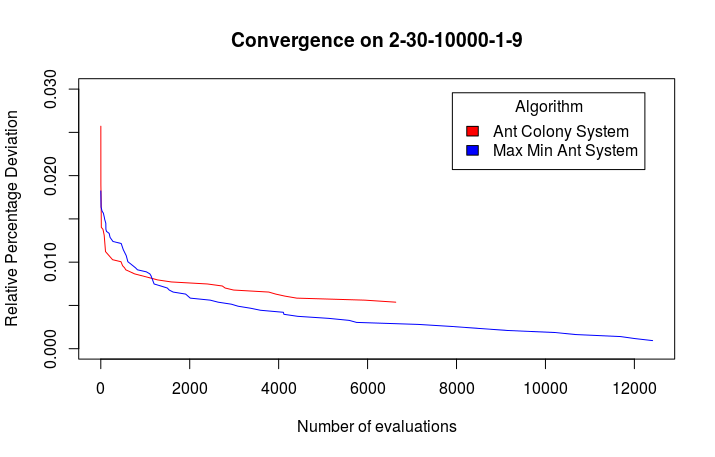
\includegraphics[scale=0.31]{conv-2-30}
            \end{figure}
        \end{column}

        \begin{column}{0.5\textwidth}
            \begin{figure}
                \centering
                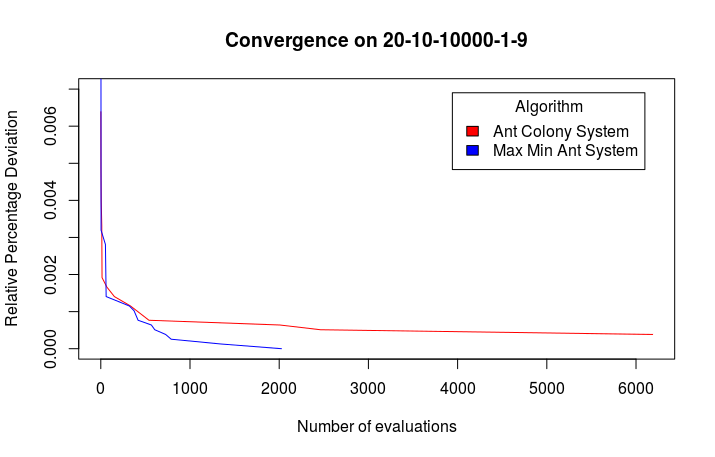
\includegraphics[scale=0.31]{conv-20-10}
            \end{figure}
        \end{column}

    \end{columns}

    \begin{itemize}
        \item Expirements with a budget of 20000 evaluations
        \item ACS seems to converge sooner
        \item However, at the very beginning, it could be better
    \end{itemize}

\end{frame}

\section{Conclusion}

\begin{frame}{Conclusion}
    \begin{itemize}
        \item Good results, high quality solution reached by both algorithms
        \item Max Min seems to reach higher quality solutions
        \item ACS seems to be more performent at the very beginning, but more tests are required
        \item A pheromones re-initialization step could be interesting for ACS
        \item More sophisticated local searches can be implemented
    \end{itemize}
\end{frame}

\begin{frame}{References}

    % \beamertemplateonlinebibitems

    \begin{thebibliography}{1}

        \bibitem{aco_csp} Simone Faro and Elisa Pappalardo.
        Ant-CSP: An Ant Colony Optimization Algorithm for the Closest String Problem, pages 370-381.
        Springer Berlin
        Heidelberg, Berlin, Heidelberg, 2010.

    \end{thebibliography}

\end{frame}


\end{document}
